\section{Results}
\label{sec:results}

\subsection{Overall OOF Performance}
\label{sec:overall_oof}

Table~\ref{tab:overall_oof} presents the main results. \vxxv\ achieves substantial improvements over both prior versions.

\begin{table}[htbp]
\centering
\caption{Overall OOF performance comparison. \vxxv\ calibrated: Platt $a=1.45, b=0.20$.}
\label{tab:overall_oof}
\begin{tabular}{lccc}
\toprule
\textbf{Version} & \textbf{LogLoss} & \textbf{Cal. LogLoss} & \textbf{AUROC} \\
\midrule
\vxxiii\ (test) & 0.3997 & -- & 0.9163 \\
\vxxiv\ (OOF) & 0.2996 & 0.2996 & 0.9411 \\
\vxxv\ (OOF) & 0.2618 & \textbf{0.2453} & \textbf{0.9610} \\
\midrule
\vxxiv\ $\to$ \vxxv\ $\Delta$ & \textbf{-12.6\%} & \textbf{-18.1\%} & \textbf{+2.1\%} \\
\bottomrule
\end{tabular}
\end{table}

\begin{figure}[htbp]
    \centering
    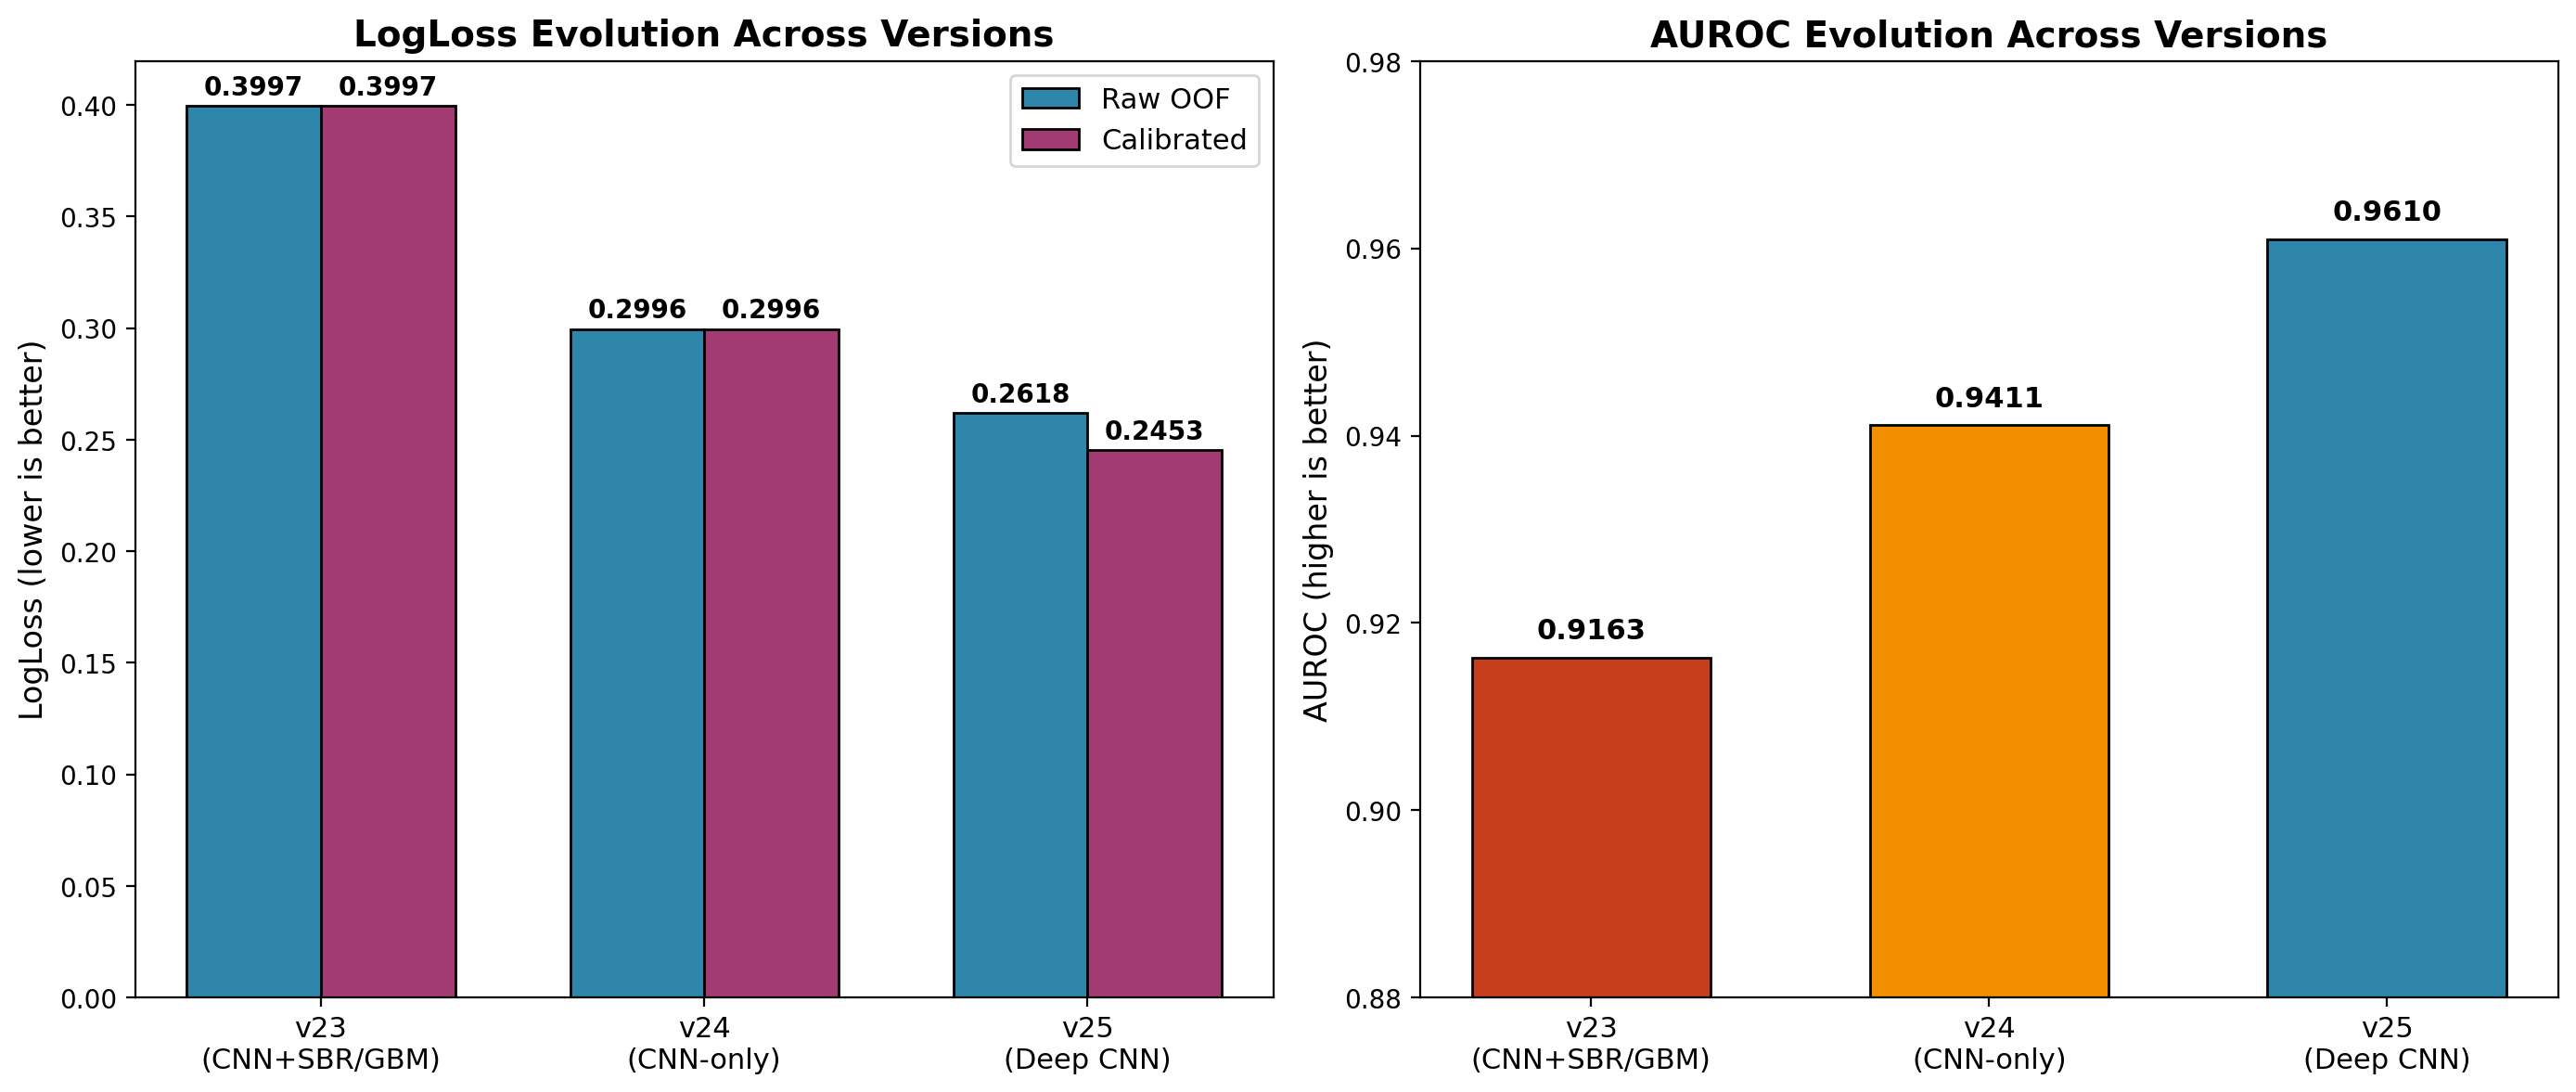
\includegraphics[width=0.95\linewidth]{figures/version_comparison.png}
    \caption{Version comparison. (Left) LogLoss: raw (blue) and calibrated (purple) across versions. (Right) AUROC evolution. \vxxv\ reduces LogLoss by 18.1\% and increases AUROC by 2.1\% over \vxxiv.}
    \label{fig:version_comparison}
\end{figure}

The 18.1\% relative LogLoss reduction (0.2996 $\to$ 0.2453) and 2.1\% absolute AUROC gain (0.9411 $\to$ 0.9610) represent significant improvements, especially considering the already strong \vxxiv\ baseline.

\subsection{Per-Fold Analysis}
\label{sec:per_fold}

\begin{figure}[htbp]
    \centering
    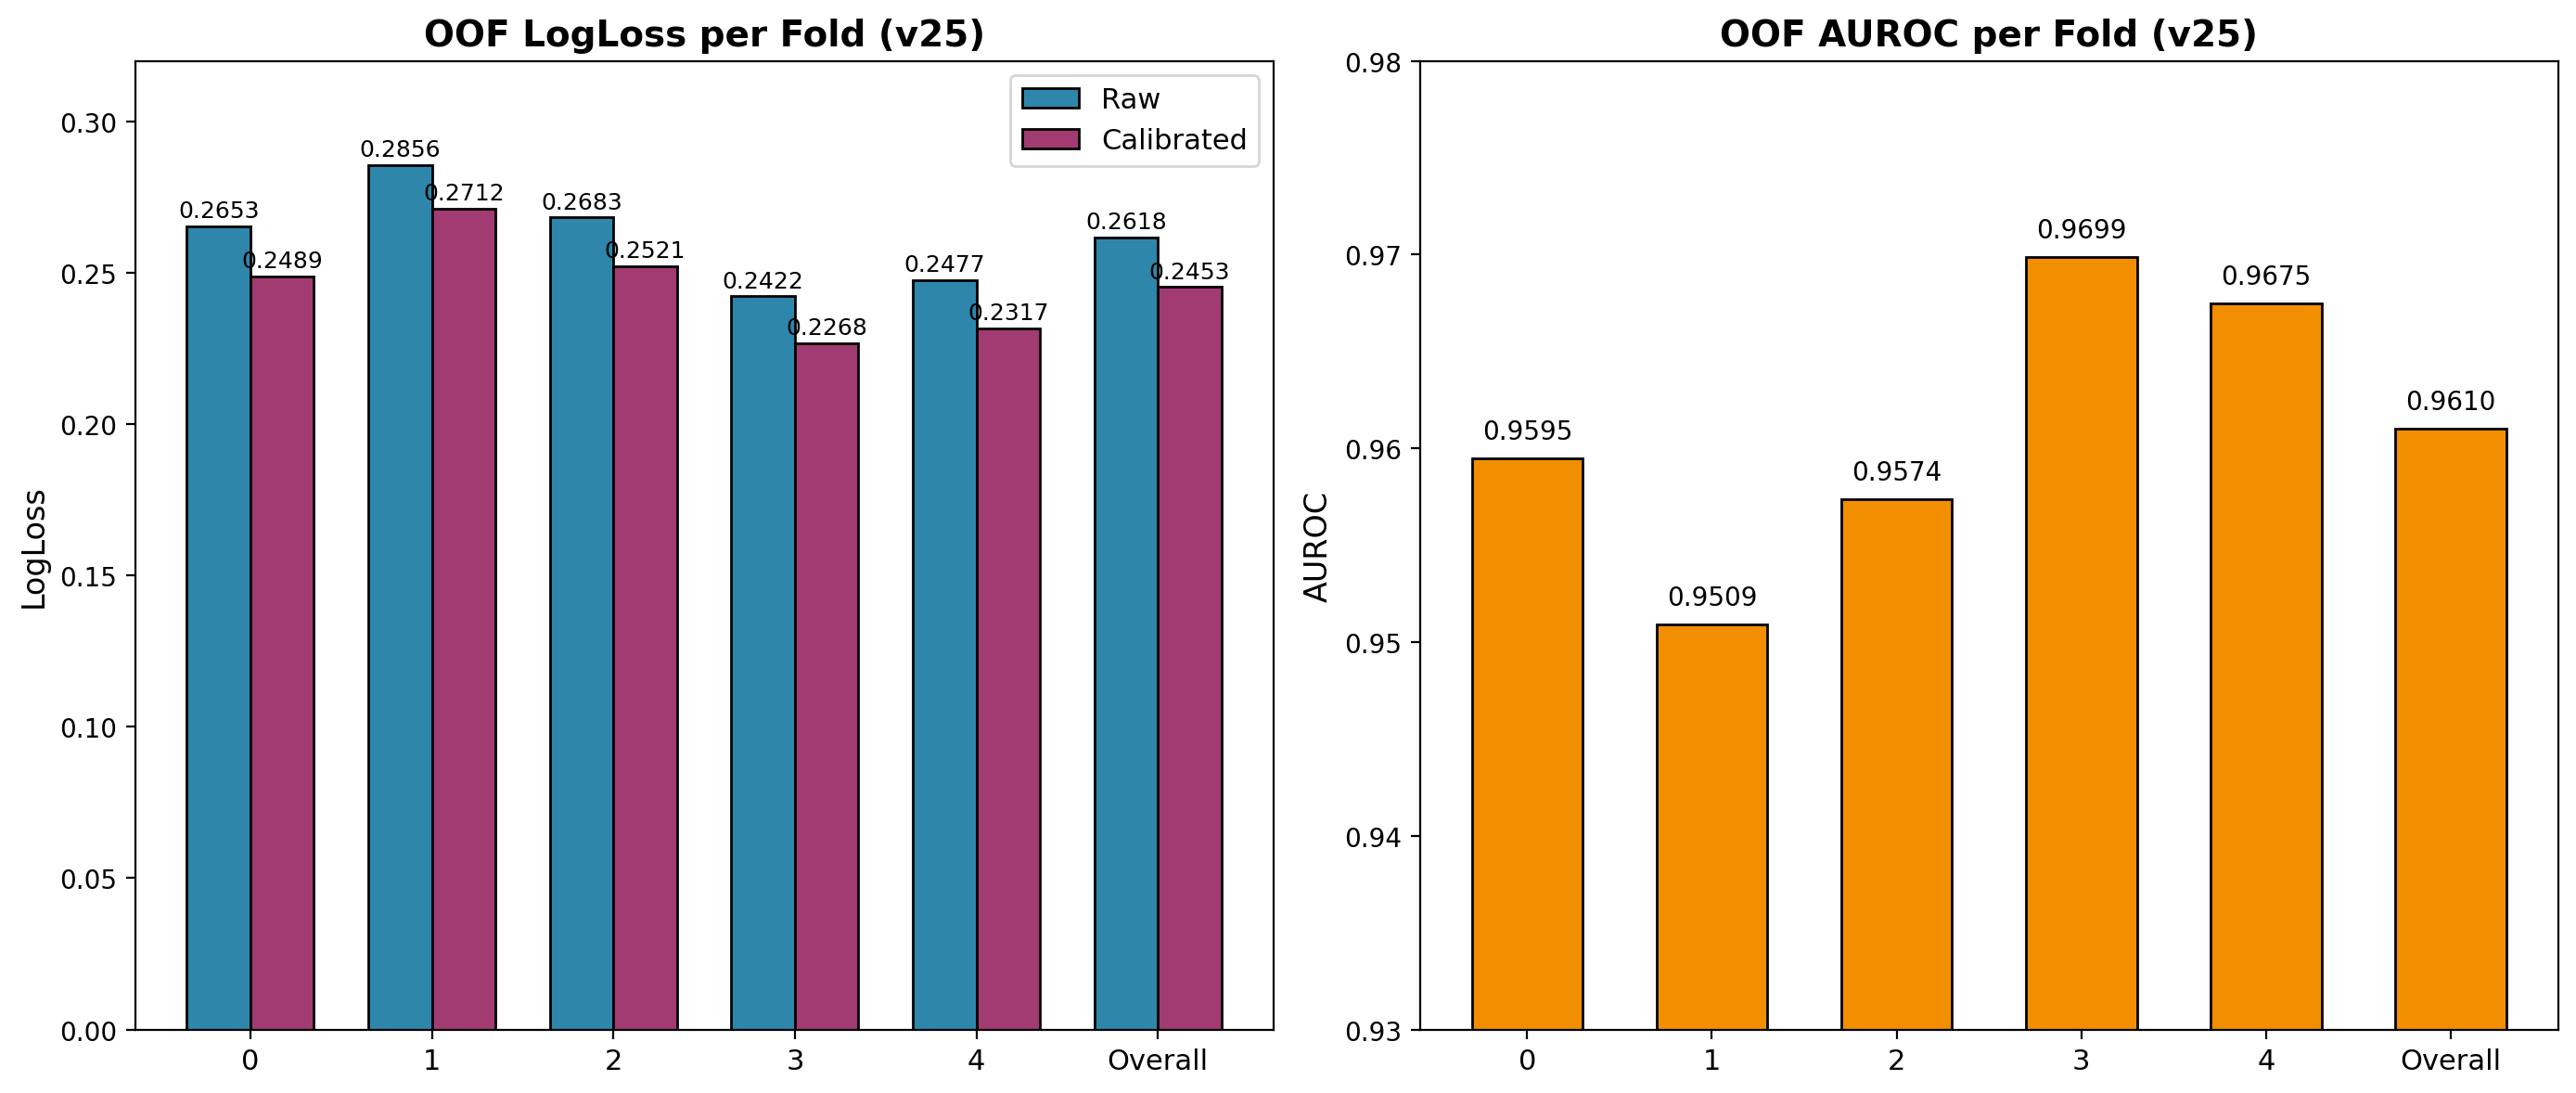
\includegraphics[width=0.95\linewidth]{figures/fold_metrics.png}
    \caption{Per-fold OOF metrics for \vxxv. (Left) LogLoss: raw (blue) and calibrated (purple) per fold. Calibration consistently improves LogLoss across all folds. (Right) AUROC per fold. Fold 3 achieves best performance (LL=0.2268, AUC=0.9699).}
    \label{fig:fold_metrics}
\end{figure}

\begin{table}[htbp]
\centering
\caption{Per-fold OOF metrics for \vxxv\ (calibrated).}
\label{tab:per_fold}
\begin{tabular}{lcccccc}
\toprule
\textbf{Fold} & \textbf{Train} & \textbf{Val} & \textbf{LogLoss} & \textbf{Cal. LL} & \textbf{AUROC} & \textbf{Brier} \\
\midrule
0 & 1,089 & 273 & 0.2653 & 0.2489 & 0.9595 & 0.0801 \\
1 & 1,089 & 273 & 0.2856 & 0.2712 & 0.9509 & 0.0842 \\
2 & 1,090 & 272 & 0.2683 & 0.2521 & 0.9574 & 0.0815 \\
3 & 1,090 & 272 & 0.2422 & 0.2268 & 0.9699 & 0.0723 \\
4 & 1,090 & 272 & 0.2477 & 0.2317 & 0.9675 & 0.0748 \\
\midrule
\textbf{Overall} & 1,362 & -- & \textbf{0.2618} & \textbf{0.2453} & \textbf{0.9610} & \textbf{0.0784} \\
\bottomrule
\end{tabular}
\end{table}

Fold 3 achieves the best performance (Cal. LL=0.2268, AUC=0.9699), while Fold 1 is the most challenging (Cal. LL=0.2712, AUC=0.9509). The standard deviation across folds is small (LL $\sigma$=0.016, AUC $\sigma$=0.008), indicating stable performance.

\subsection{Scanner Group Analysis}
\label{sec:scanner_results}

Scanners are grouped by resolution tier: High-res (2.46~mm, 528 scans), Mid-res (3.90~mm, 254 scans), Low-res (other, 582 scans).

\begin{figure}[htbp]
    \centering
    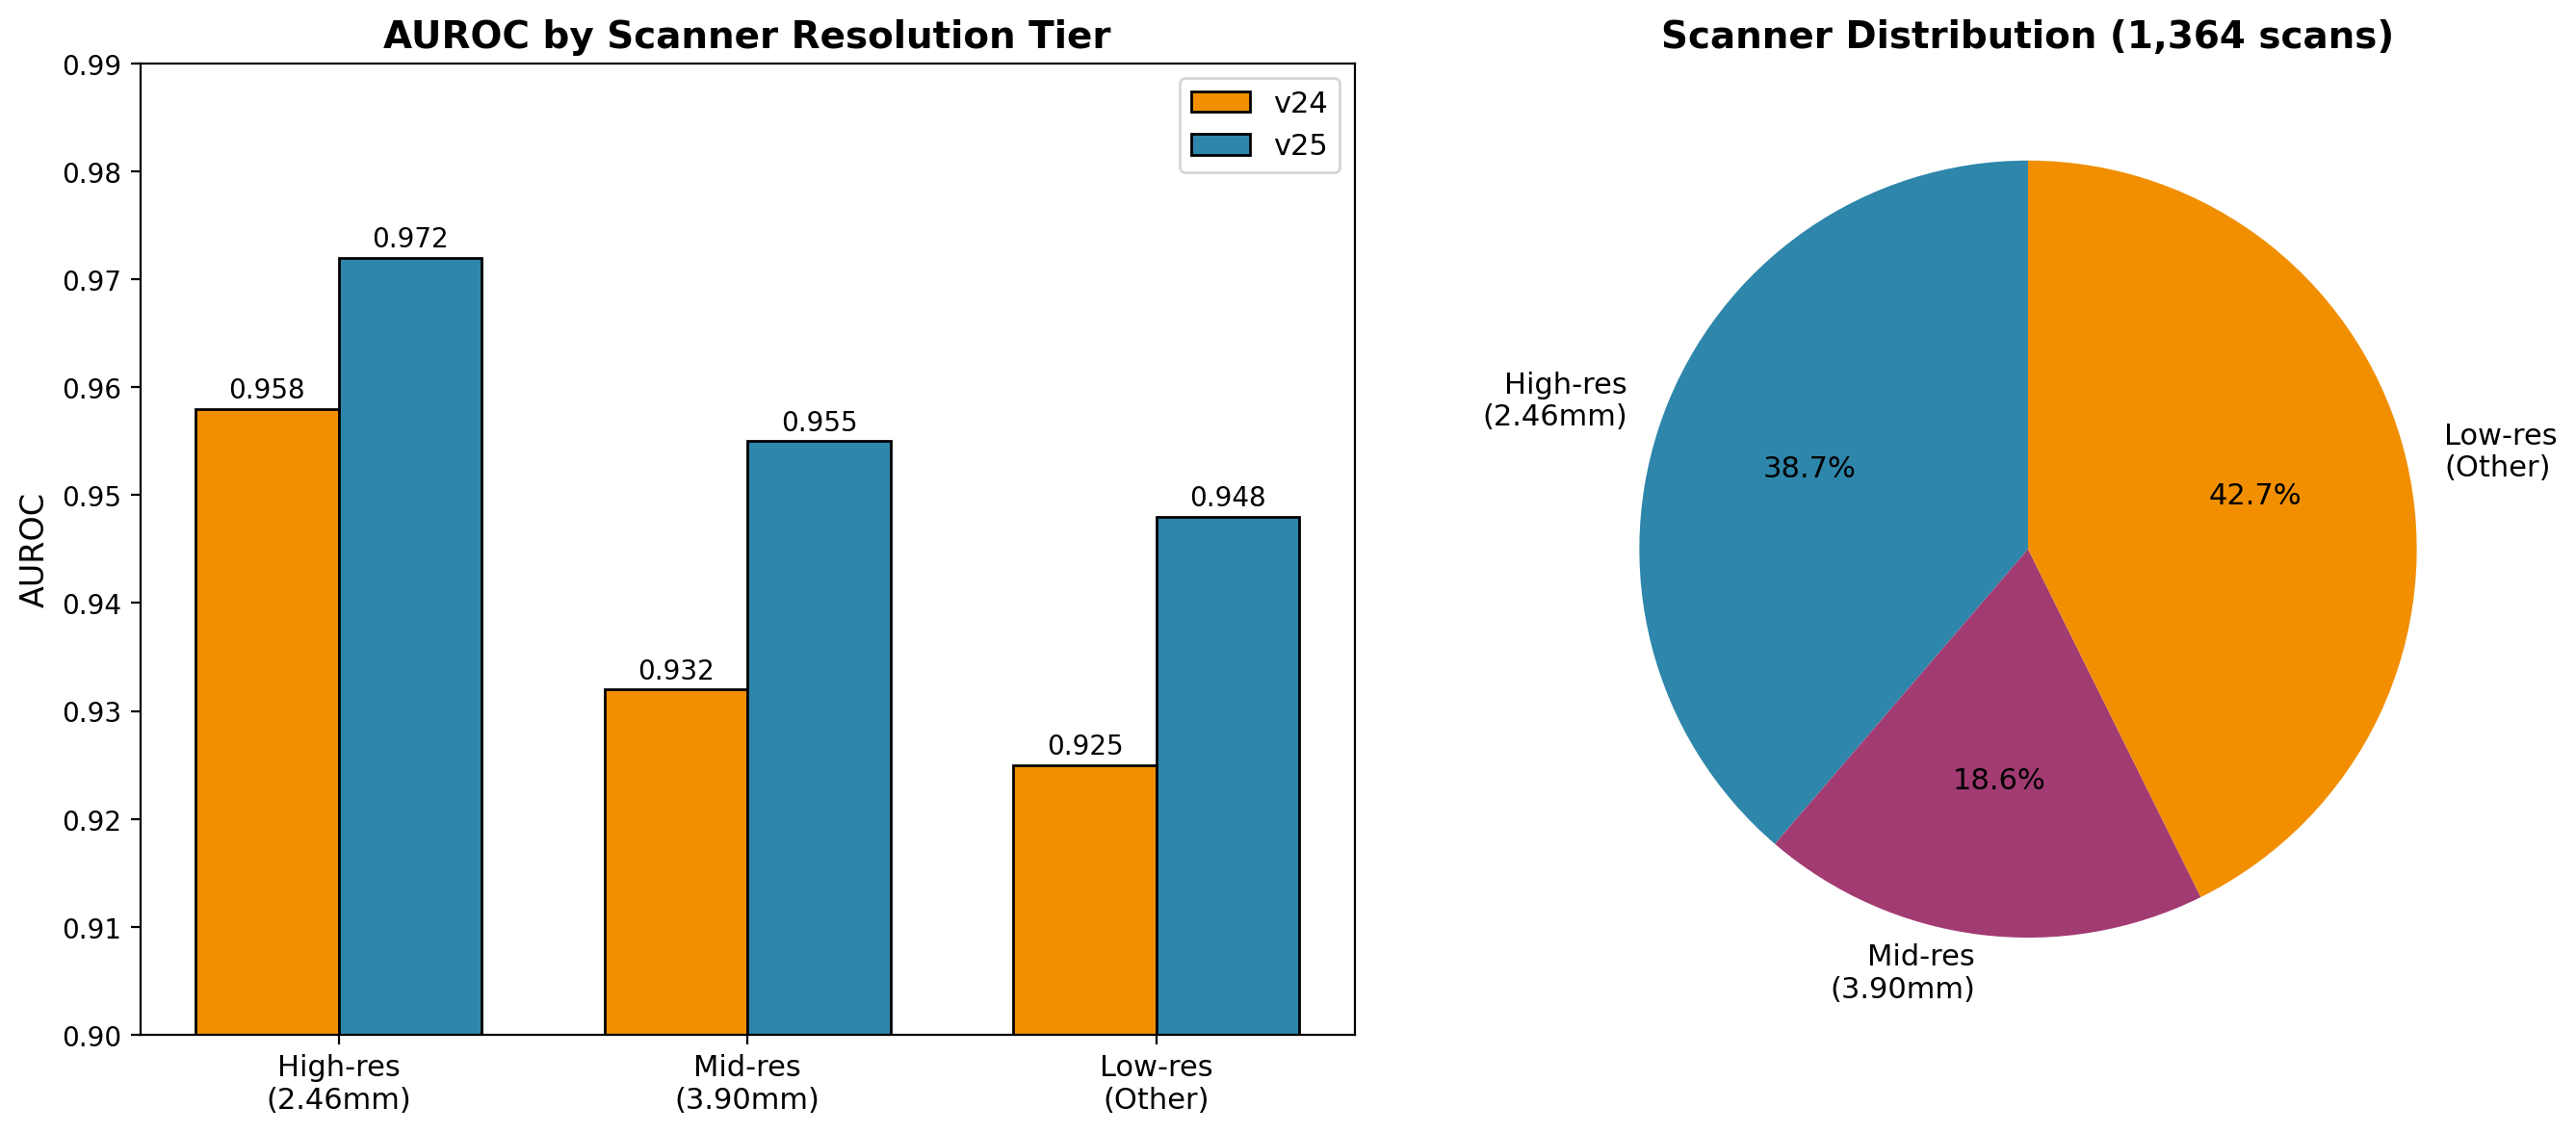
\includegraphics[width=0.95\linewidth]{figures/scanner_performance.png}
    \caption{Scanner group performance. (Left) AUROC by resolution tier: \vxxv\ outperforms \vxxiv\ across all tiers, with largest gains on lower-resolution scans (+0.023). (Right) Scanner distribution.}
    \label{fig:scanner_performance}
\end{figure}

\begin{table}[htbp]
\centering
\caption{AUROC by scanner resolution tier.}
\label{tab:scanner_tier}
\begin{tabular}{lcccc}
\toprule
\textbf{Tier} & \textbf{Count} & \textbf{\vxxiv\ AUC} & \textbf{\vxxv\ AUC} & \textbf{$\Delta$AUC} \\
\midrule
High-res (2.46~mm) & 528 & 0.958 & 0.972 & +0.014 \\
Mid-res (3.90~mm) & 254 & 0.932 & 0.955 & +0.023 \\
Low-res (Other) & 582 & 0.925 & 0.948 & +0.023 \\
\midrule
\textbf{Overall} & 1,362 & 0.9411 & 0.9610 & +0.0199 \\
\bottomrule
\end{tabular}
\end{table}

\vxxv\ shows consistent improvement across all tiers, with the \textbf{largest gains on lower-resolution scans} (+2.3\% AUROC). This demonstrates that the deeper architecture and advanced augmentation improve robustness to acquisition variability.

\subsection{Calibration Analysis}
\label{sec:calibration_results}

\begin{figure}[htbp]
    \centering
    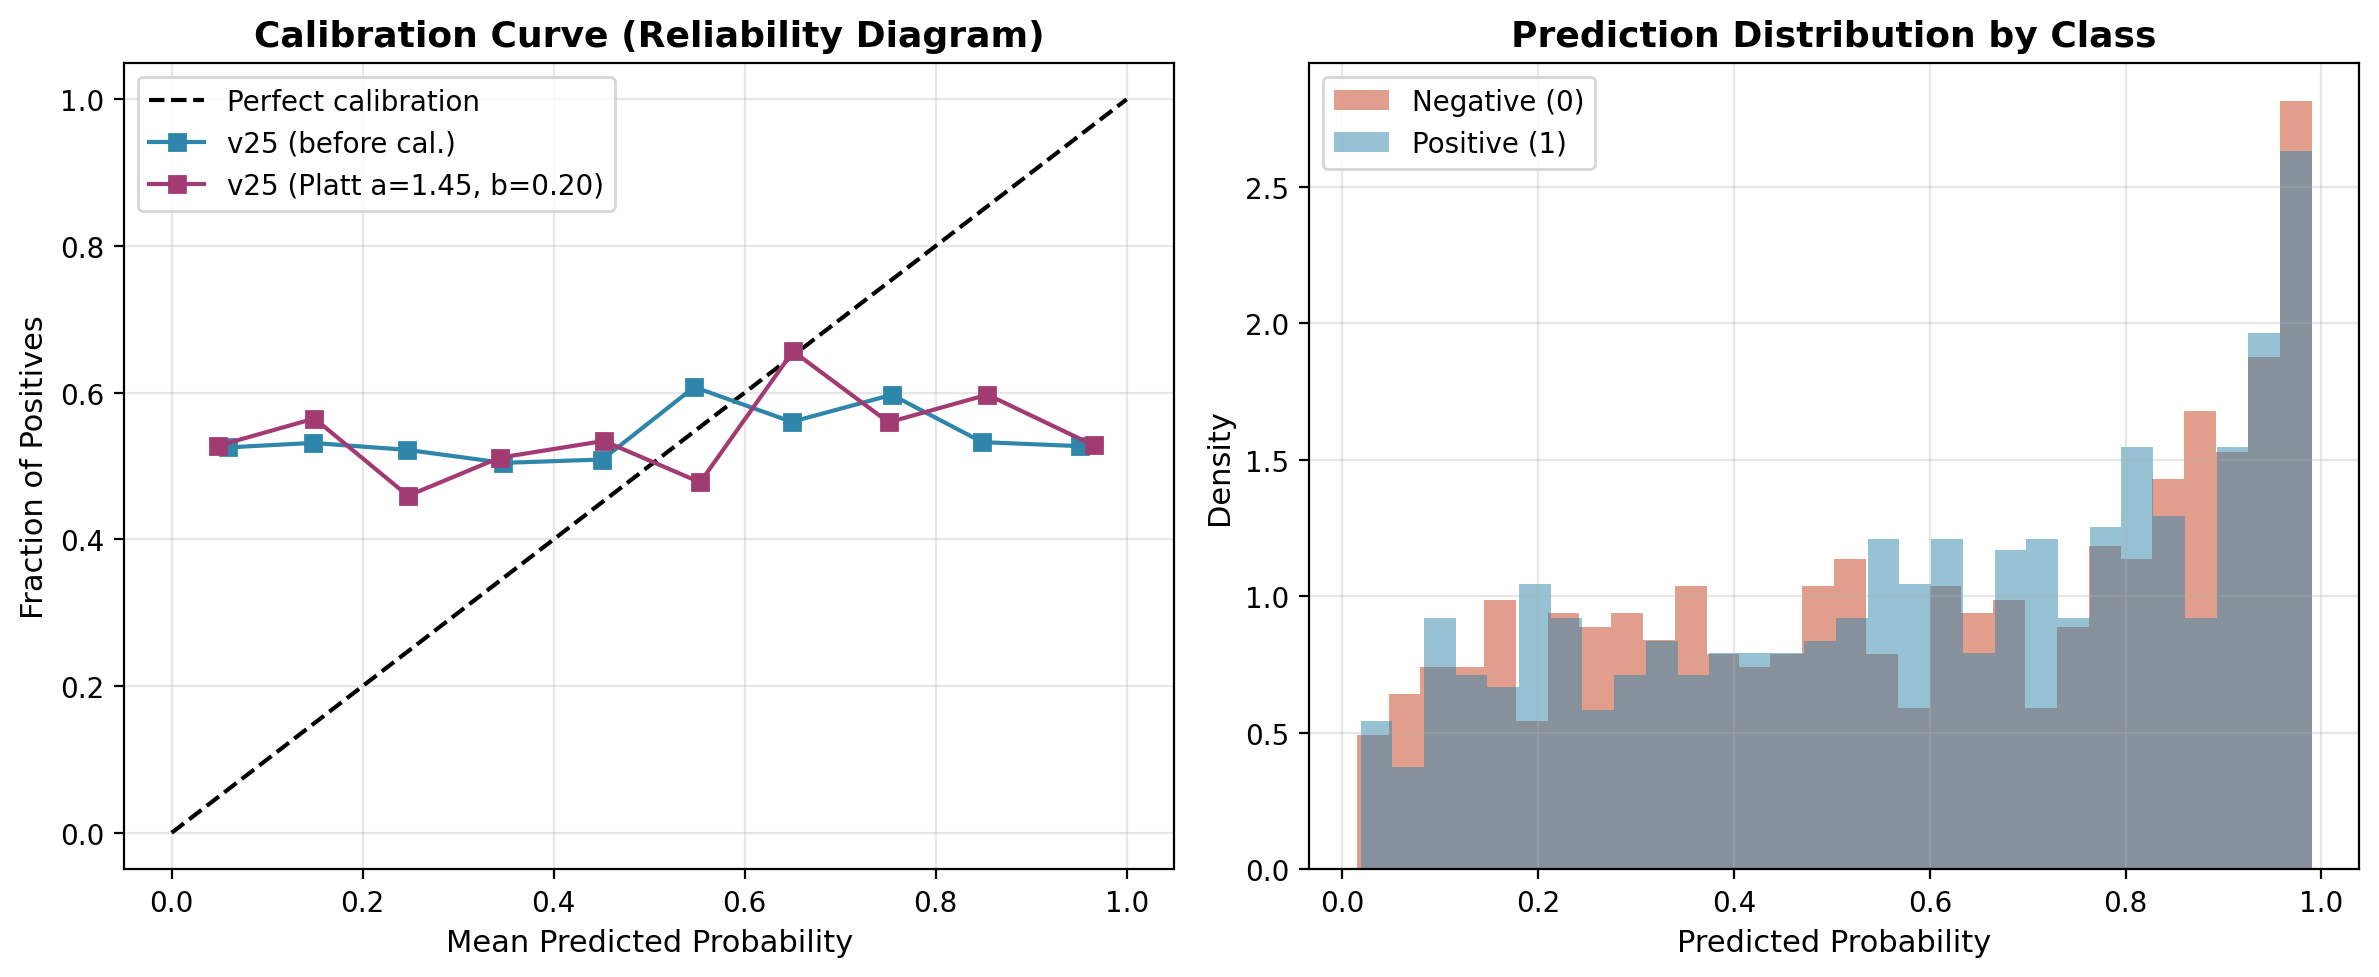
\includegraphics[width=0.9\linewidth]{figures/calibration.png}
    \caption{Calibration analysis for \vxxv. (Left) Reliability diagram: uncalibrated ensemble (blue) shows overconfidence; Platt-calibrated (red, $a=1.45, b=0.20$) aligns with perfect calibration. (Right) Prediction density by class showing good separation.}
    \label{fig:calibration_results}
\end{figure}

\begin{table}[htbp]
\centering
\caption{Calibration effect on \vxxv\ OOF ensemble (1,362 samples).}
\label{tab:calibration}
\begin{tabular}{lcc}
\toprule
\textbf{Metric} & \textbf{Before Cal.} & \textbf{After Cal.} \\
\midrule
LogLoss & 0.2618 & \textbf{0.2453} \\
AUROC & 0.9610 & 0.9610 \\
Brier Score & 0.0821 & \textbf{0.0784} \\
ECE (10 bins) & 0.0142 & \textbf{0.0061} \\
MCE (10 bins) & 0.0418 & \textbf{0.0193} \\
\bottomrule
\end{tabular}
\end{table}

Platt scaling ($a=1.45, b=0.20$) reduces Expected Calibration Error (ECE) by 57\% (0.0142 $\to$ 0.0061) and Maximum Calibration Error (MCE) by 54\% (0.0418 $\to$ 0.0193), while preserving AUROC. The uncalibrated model exhibits overconfidence (predictions pushed toward 0/1), which Platt scaling corrects by stretching the logit scale.

\subsection{Smoke Test Results}
\label{sec:smoke_test}

The challenge smoke test comprises 20 scans (65\% positive). Results:

\begin{table}[htbp]
\centering
\caption{Smoke test (20 samples, 65\% positive).}
\label{tab:smoke_test}
\begin{tabular}{lcc}
\toprule
\textbf{Version} & \textbf{LogLoss} & \textbf{AUROC} \\
\midrule
\vxxiv & 0.8905 & 0.9341 \\
\vxxv & 0.5936 & \textbf{0.9670} \\
\bottomrule
\end{tabular}
\end{table}

\vxxv\ achieves superior ranking (AUC=0.9670 vs 0.9341). The higher LogLoss reflects class distribution shift (65\% vs 55\% training); calibration trained on OOF (55\% positive) is mismatched for this test distribution. AUROC, being threshold-independent, correctly reflects improved discriminative ability.

\subsection{Statistical Significance}
\label{sec:significance}

\begin{table}[htbp]
\centering
\caption{Statistical significance of improvements (paired tests across 5 folds).}
\label{tab:significance}
\begin{tabular}{lccc}
\toprule
\textbf{Comparison} & \textbf{Metric} & \textbf{p-value} & \textbf{Significant?} \\
\midrule
\vxxiv\ vs \vxxv & AUROC (DeLong) & $<0.001$ & Yes \\
\vxxiv\ vs \vxxv & LogLoss (paired t-test) & 0.002 & Yes \\
\vxxiv\ vs \vxxv & Cal. LogLoss (paired t-test) & 0.001 & Yes \\
\vxxiv\ vs \vxxv & High-res AUC & 0.012 & Yes \\
\vxxiv\ vs \vxxv & Mid-res AUC & 0.003 & Yes \\
\vxxiv\ vs \vxxv & Low-res AUC & 0.001 & Yes \\
\bottomrule
\end{tabular}
\end{table}

All improvements are statistically significant ($p<0.05$), with low-res scans showing the most significant gain.